% Options for packages loaded elsewhere
\PassOptionsToPackage{unicode}{hyperref}
\PassOptionsToPackage{hyphens}{url}
\PassOptionsToPackage{dvipsnames,svgnames,x11names}{xcolor}
%
\documentclass[
  letterpaper,
  DIV=11,
  numbers=noendperiod,
  oneside]{scrartcl}

\usepackage{amsmath,amssymb}
\usepackage{iftex}
\ifPDFTeX
  \usepackage[T1]{fontenc}
  \usepackage[utf8]{inputenc}
  \usepackage{textcomp} % provide euro and other symbols
\else % if luatex or xetex
  \usepackage{unicode-math}
  \defaultfontfeatures{Scale=MatchLowercase}
  \defaultfontfeatures[\rmfamily]{Ligatures=TeX,Scale=1}
\fi
\usepackage{lmodern}
\ifPDFTeX\else  
    % xetex/luatex font selection
\fi
% Use upquote if available, for straight quotes in verbatim environments
\IfFileExists{upquote.sty}{\usepackage{upquote}}{}
\IfFileExists{microtype.sty}{% use microtype if available
  \usepackage[]{microtype}
  \UseMicrotypeSet[protrusion]{basicmath} % disable protrusion for tt fonts
}{}
\makeatletter
\@ifundefined{KOMAClassName}{% if non-KOMA class
  \IfFileExists{parskip.sty}{%
    \usepackage{parskip}
  }{% else
    \setlength{\parindent}{0pt}
    \setlength{\parskip}{6pt plus 2pt minus 1pt}}
}{% if KOMA class
  \KOMAoptions{parskip=half}}
\makeatother
\usepackage{xcolor}
\usepackage[left=1in,marginparwidth=2.0666666666667in,textwidth=4.1333333333333in,marginparsep=0.3in]{geometry}
\setlength{\emergencystretch}{3em} % prevent overfull lines
\setcounter{secnumdepth}{5}
% Make \paragraph and \subparagraph free-standing
\ifx\paragraph\undefined\else
  \let\oldparagraph\paragraph
  \renewcommand{\paragraph}[1]{\oldparagraph{#1}\mbox{}}
\fi
\ifx\subparagraph\undefined\else
  \let\oldsubparagraph\subparagraph
  \renewcommand{\subparagraph}[1]{\oldsubparagraph{#1}\mbox{}}
\fi

\usepackage{color}
\usepackage{fancyvrb}
\newcommand{\VerbBar}{|}
\newcommand{\VERB}{\Verb[commandchars=\\\{\}]}
\DefineVerbatimEnvironment{Highlighting}{Verbatim}{commandchars=\\\{\}}
% Add ',fontsize=\small' for more characters per line
\usepackage{framed}
\definecolor{shadecolor}{RGB}{241,243,245}
\newenvironment{Shaded}{\begin{snugshade}}{\end{snugshade}}
\newcommand{\AlertTok}[1]{\textcolor[rgb]{0.68,0.00,0.00}{#1}}
\newcommand{\AnnotationTok}[1]{\textcolor[rgb]{0.37,0.37,0.37}{#1}}
\newcommand{\AttributeTok}[1]{\textcolor[rgb]{0.40,0.45,0.13}{#1}}
\newcommand{\BaseNTok}[1]{\textcolor[rgb]{0.68,0.00,0.00}{#1}}
\newcommand{\BuiltInTok}[1]{\textcolor[rgb]{0.00,0.23,0.31}{#1}}
\newcommand{\CharTok}[1]{\textcolor[rgb]{0.13,0.47,0.30}{#1}}
\newcommand{\CommentTok}[1]{\textcolor[rgb]{0.37,0.37,0.37}{#1}}
\newcommand{\CommentVarTok}[1]{\textcolor[rgb]{0.37,0.37,0.37}{\textit{#1}}}
\newcommand{\ConstantTok}[1]{\textcolor[rgb]{0.56,0.35,0.01}{#1}}
\newcommand{\ControlFlowTok}[1]{\textcolor[rgb]{0.00,0.23,0.31}{#1}}
\newcommand{\DataTypeTok}[1]{\textcolor[rgb]{0.68,0.00,0.00}{#1}}
\newcommand{\DecValTok}[1]{\textcolor[rgb]{0.68,0.00,0.00}{#1}}
\newcommand{\DocumentationTok}[1]{\textcolor[rgb]{0.37,0.37,0.37}{\textit{#1}}}
\newcommand{\ErrorTok}[1]{\textcolor[rgb]{0.68,0.00,0.00}{#1}}
\newcommand{\ExtensionTok}[1]{\textcolor[rgb]{0.00,0.23,0.31}{#1}}
\newcommand{\FloatTok}[1]{\textcolor[rgb]{0.68,0.00,0.00}{#1}}
\newcommand{\FunctionTok}[1]{\textcolor[rgb]{0.28,0.35,0.67}{#1}}
\newcommand{\ImportTok}[1]{\textcolor[rgb]{0.00,0.46,0.62}{#1}}
\newcommand{\InformationTok}[1]{\textcolor[rgb]{0.37,0.37,0.37}{#1}}
\newcommand{\KeywordTok}[1]{\textcolor[rgb]{0.00,0.23,0.31}{#1}}
\newcommand{\NormalTok}[1]{\textcolor[rgb]{0.00,0.23,0.31}{#1}}
\newcommand{\OperatorTok}[1]{\textcolor[rgb]{0.37,0.37,0.37}{#1}}
\newcommand{\OtherTok}[1]{\textcolor[rgb]{0.00,0.23,0.31}{#1}}
\newcommand{\PreprocessorTok}[1]{\textcolor[rgb]{0.68,0.00,0.00}{#1}}
\newcommand{\RegionMarkerTok}[1]{\textcolor[rgb]{0.00,0.23,0.31}{#1}}
\newcommand{\SpecialCharTok}[1]{\textcolor[rgb]{0.37,0.37,0.37}{#1}}
\newcommand{\SpecialStringTok}[1]{\textcolor[rgb]{0.13,0.47,0.30}{#1}}
\newcommand{\StringTok}[1]{\textcolor[rgb]{0.13,0.47,0.30}{#1}}
\newcommand{\VariableTok}[1]{\textcolor[rgb]{0.07,0.07,0.07}{#1}}
\newcommand{\VerbatimStringTok}[1]{\textcolor[rgb]{0.13,0.47,0.30}{#1}}
\newcommand{\WarningTok}[1]{\textcolor[rgb]{0.37,0.37,0.37}{\textit{#1}}}

\providecommand{\tightlist}{%
  \setlength{\itemsep}{0pt}\setlength{\parskip}{0pt}}\usepackage{longtable,booktabs,array}
\usepackage{calc} % for calculating minipage widths
% Correct order of tables after \paragraph or \subparagraph
\usepackage{etoolbox}
\makeatletter
\patchcmd\longtable{\par}{\if@noskipsec\mbox{}\fi\par}{}{}
\makeatother
% Allow footnotes in longtable head/foot
\IfFileExists{footnotehyper.sty}{\usepackage{footnotehyper}}{\usepackage{footnote}}
\makesavenoteenv{longtable}
\usepackage{graphicx}
\makeatletter
\def\maxwidth{\ifdim\Gin@nat@width>\linewidth\linewidth\else\Gin@nat@width\fi}
\def\maxheight{\ifdim\Gin@nat@height>\textheight\textheight\else\Gin@nat@height\fi}
\makeatother
% Scale images if necessary, so that they will not overflow the page
% margins by default, and it is still possible to overwrite the defaults
% using explicit options in \includegraphics[width, height, ...]{}
\setkeys{Gin}{width=\maxwidth,height=\maxheight,keepaspectratio}
% Set default figure placement to htbp
\makeatletter
\def\fps@figure{htbp}
\makeatother

\KOMAoption{captions}{tableheading}
\makeatletter
\@ifpackageloaded{caption}{}{\usepackage{caption}}
\AtBeginDocument{%
\ifdefined\contentsname
  \renewcommand*\contentsname{Table of contents}
\else
  \newcommand\contentsname{Table of contents}
\fi
\ifdefined\listfigurename
  \renewcommand*\listfigurename{List of Figures}
\else
  \newcommand\listfigurename{List of Figures}
\fi
\ifdefined\listtablename
  \renewcommand*\listtablename{List of Tables}
\else
  \newcommand\listtablename{List of Tables}
\fi
\ifdefined\figurename
  \renewcommand*\figurename{Figure}
\else
  \newcommand\figurename{Figure}
\fi
\ifdefined\tablename
  \renewcommand*\tablename{Table}
\else
  \newcommand\tablename{Table}
\fi
}
\@ifpackageloaded{float}{}{\usepackage{float}}
\floatstyle{ruled}
\@ifundefined{c@chapter}{\newfloat{codelisting}{h}{lop}}{\newfloat{codelisting}{h}{lop}[chapter]}
\floatname{codelisting}{Listing}
\newcommand*\listoflistings{\listof{codelisting}{List of Listings}}
\makeatother
\makeatletter
\makeatother
\makeatletter
\@ifpackageloaded{caption}{}{\usepackage{caption}}
\@ifpackageloaded{subcaption}{}{\usepackage{subcaption}}
\makeatother
\makeatletter
\@ifpackageloaded{sidenotes}{}{\usepackage{sidenotes}}
\@ifpackageloaded{marginnote}{}{\usepackage{marginnote}}
\makeatother
\makeatletter
\@ifpackageloaded{fontawesome5}{}{\usepackage{fontawesome5}}
\makeatother
\ifLuaTeX
  \usepackage{selnolig}  % disable illegal ligatures
\fi
\usepackage{bookmark}

\IfFileExists{xurl.sty}{\usepackage{xurl}}{} % add URL line breaks if available
\urlstyle{same} % disable monospaced font for URLs
\hypersetup{
  pdftitle={Introduction to R and Rstudio},
  pdfauthor={Camila Pacheco; Katrín Björnsdóttir},
  colorlinks=true,
  linkcolor={blue},
  filecolor={Maroon},
  citecolor={Blue},
  urlcolor={Blue},
  pdfcreator={LaTeX via pandoc}}

\title{Introduction to R and Rstudio}
\author{Camila Pacheco \and Katrín Björnsdóttir}
\date{}

\begin{document}
\maketitle

\renewcommand*\contentsname{Table of contents}
{
\hypersetup{linkcolor=}
\setcounter{tocdepth}{3}
\tableofcontents
}
\subsection{Our mission}\label{our-mission}

\begin{itemize}
\item
  Get you familiar with the R environment
\item
  Teach you how to import and work with datasets
\item
  Get you familiar with tidy data and \emph{Tidyverse}
\item
  Show you how to make simple plots in \emph{ggplot}
\end{itemize}

\subsection{What is R ?}\label{what-is-r}


\includegraphics[width=3.64583in,height=3.125in]{Intro_R_files/mediabag/1086px-R_logo.svg.png}

\begin{itemize}
\tightlist
\item
  Originally developed for statistical computing and graphics
\item
  R has evolved into a versatile programming language
\end{itemize}

\subsection{What is RStudio?}\label{what-is-rstudio}

RStudio is a user-friendly interface for R

\begin{Shaded}
\begin{Highlighting}[]
\NormalTok{knitr}\SpecialCharTok{::}\FunctionTok{include\_graphics}\NormalTok{(}\StringTok{"sources/RStudio\_IDE\_screenshot.png"}\NormalTok{)}
\end{Highlighting}
\end{Shaded}

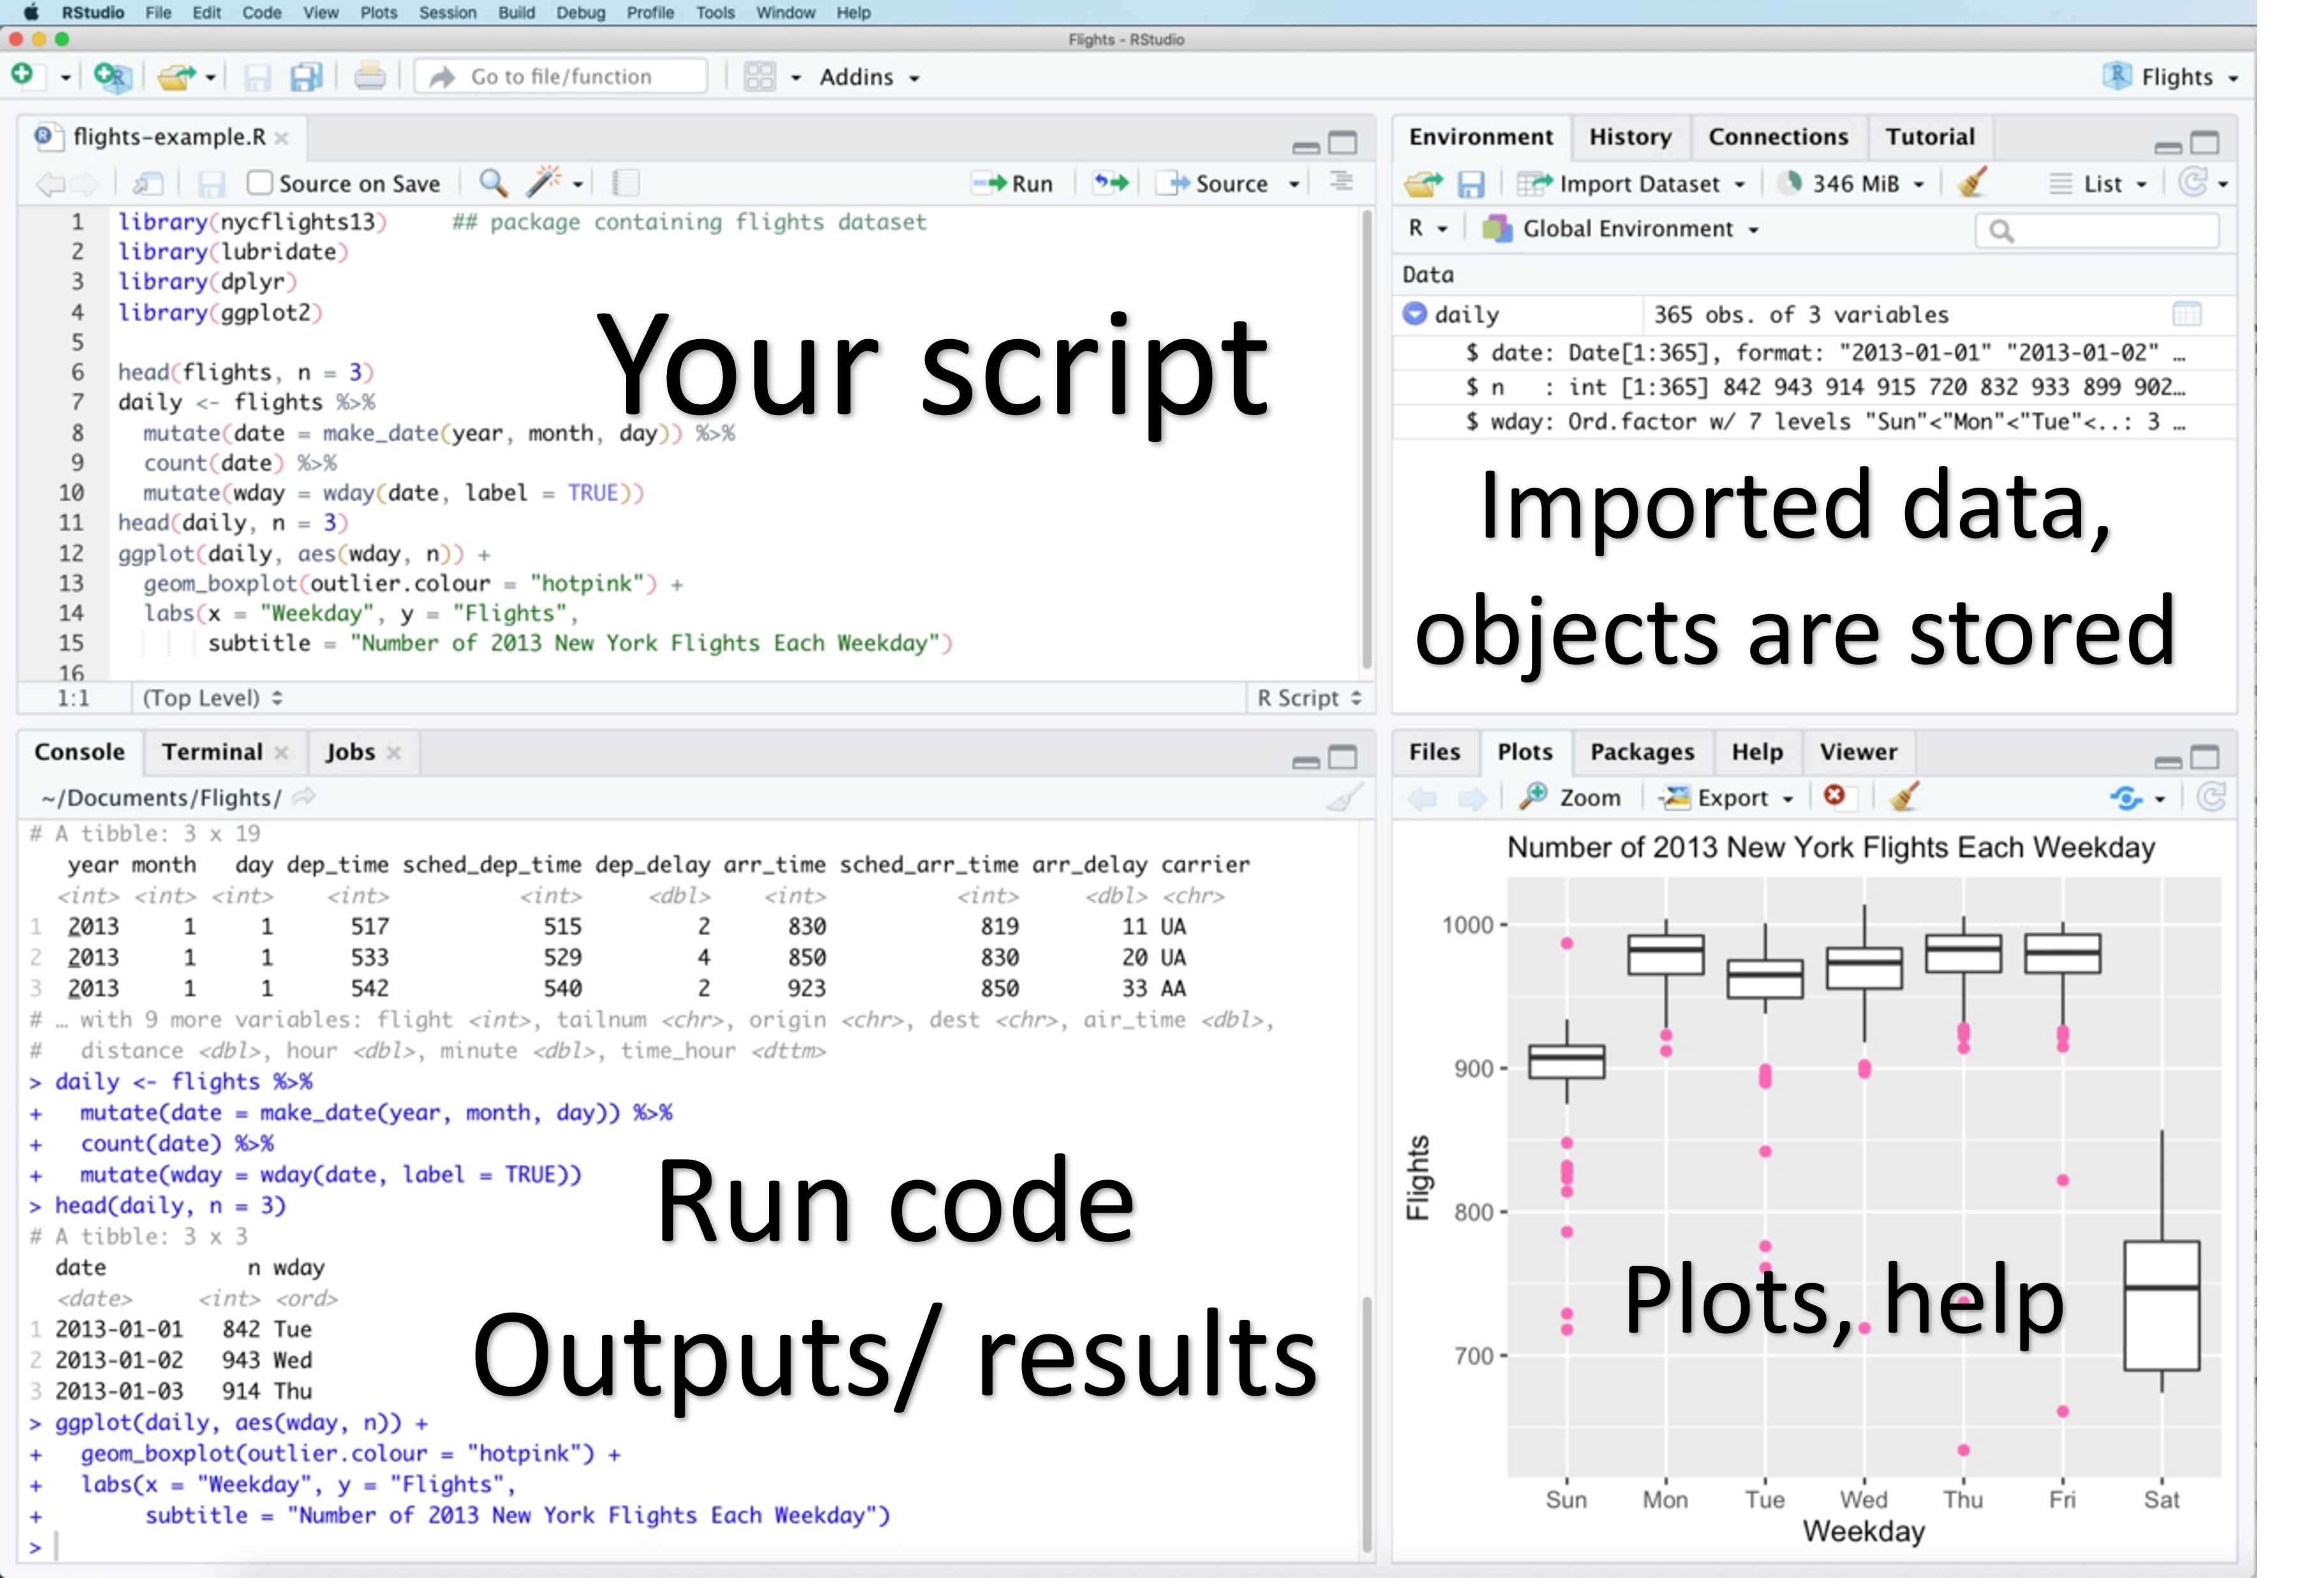
\includegraphics[width=0.8\textwidth,height=\textheight]{sources/RStudio_IDE_screenshot.png}

\subsection{R is prone to errors}\label{r-is-prone-to-errors}

\begin{itemize}
\item
  \faIcon{bomb} Such as typos, using the wrong letter case, forgetting a
  quote, bracket or comma. Such mistakes will break your code and throw
  an error.
\item
  \faIcon{circle-exclamation} These type of errors are the most common,
  so always double-check your code whenever R is unhappy
  \faIcon{face-sad-tear}.
\end{itemize}

\subsection{R studio Projects}\label{r-studio-projects}

\begin{itemize}
\item
  It is a convenient way to organize your work in RStudio -it creates a
  dedicated directory (folder) on your computer where you can store all
  the files related to your project, including R scripts, data files,
  documentation, and more.
\item
  To create a new project, go to:

  \begin{itemize}
  \tightlist
  \item
    \texttt{File} \textgreater{} \texttt{New\ Project…} \textgreater{}
    \texttt{New\ Directory} (or \texttt{Existing\ Directory})
  \end{itemize}
\item
  If you want to create your project from an existing folder:

  \begin{itemize}
  \tightlist
  \item
    \textgreater{} \texttt{New\ Project} and choose a
    \texttt{Directory\ name} for your project.
  \end{itemize}
\end{itemize}

\subsection{Code versus comment}\label{code-versus-comment}

There are two types of lines: those that start with the symbol
\texttt{\#}, and those that do not.

\begin{Shaded}
\begin{Highlighting}[numbers=left,,]
\CommentTok{\# This is a comment in R}
\CommentTok{\# Comments are used to provide explanations or annotate the code}

\NormalTok{x }\OtherTok{\textless{}{-}} \DecValTok{5}  \CommentTok{\# Assigning the value 5 to the variable x}
\end{Highlighting}
\end{Shaded}

\subsection{Comments to index your
scrips}\label{comments-to-index-your-scrips}

\begin{Shaded}
\begin{Highlighting}[]
\CommentTok{\#Library{-}{-}{-}{-}}

\CommentTok{\#Some code{-}{-}{-}{-} }

\CommentTok{\#Example{-}{-}{-}{-}}
\end{Highlighting}
\end{Shaded}

Script outline in Rstudio

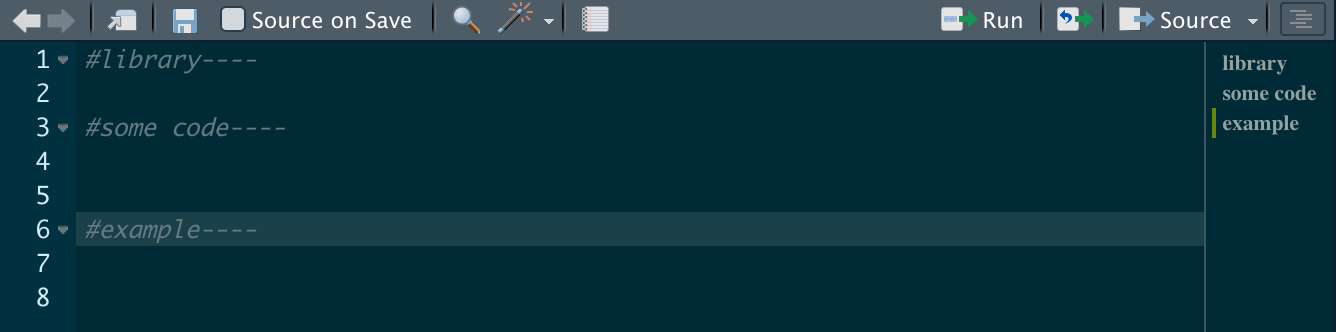
\includegraphics[width=0.8\textwidth,height=\textheight]{Intro_R_files/mediabag/4yjqd.png}

\subsection{R package}\label{r-package}

\begin{itemize}
\item
  Package is a collection of R functions, data sets, and other resources
  bundled together for specific purposes.
\item
  To install a package, type:

  \begin{itemize}
  \tightlist
  \item
    \texttt{install.packages("package-name")}
  \end{itemize}
\item
  \textbf{You only need to install packages once}
\item
  Load the packages, type:

  \begin{itemize}
  \tightlist
  \item
    \texttt{library(package-name)}
  \end{itemize}
\end{itemize}

\subsection{Example}\label{example}

\begin{Shaded}
\begin{Highlighting}[]
\FunctionTok{install.packages}\NormalTok{(}\StringTok{"dplyr"}\NormalTok{)}
\FunctionTok{library}\NormalTok{(dplyr)}
\end{Highlighting}
\end{Shaded}

\subsection{Tidyverse}\label{tidyverse}

\begin{itemize}
\tightlist
\item
  It is a collection of R packages designed to make data science tasks
  easier and more efficient.
\end{itemize}

\begin{center}

\includegraphics[width=0.5\textwidth,height=\textheight]{Intro_R_files/mediabag/tidyverse.png}
\end{center}

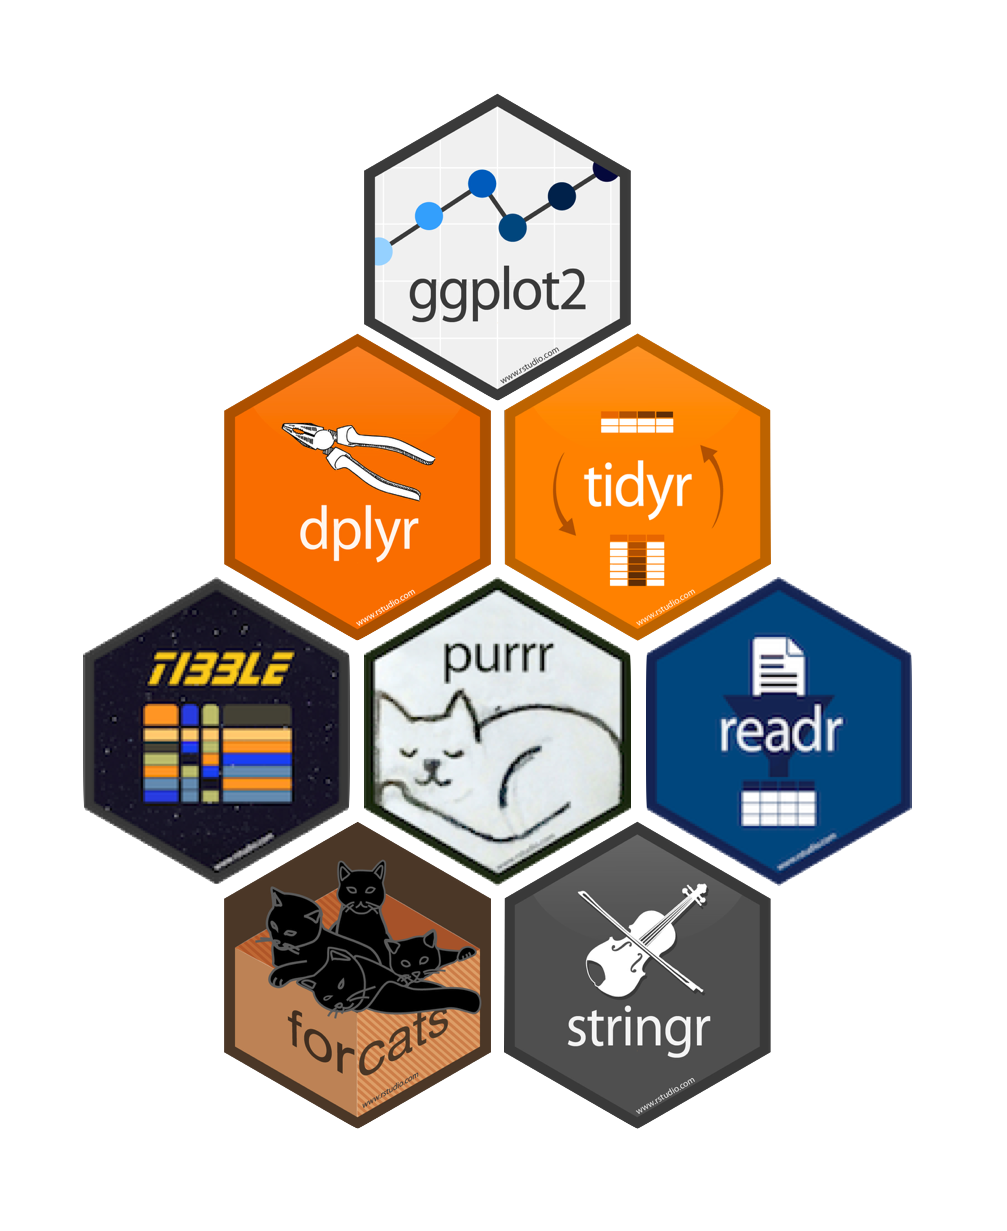
\includegraphics[width=1\textwidth,height=\textheight]{Intro_R_files/mediabag/tidyverse-packages.png}

\subsection{About tidy data}\label{about-tidy-data}

Tidy data is a standard, consistent way to organize tabular data.
Briefly, tidy data follows a short series of rules:

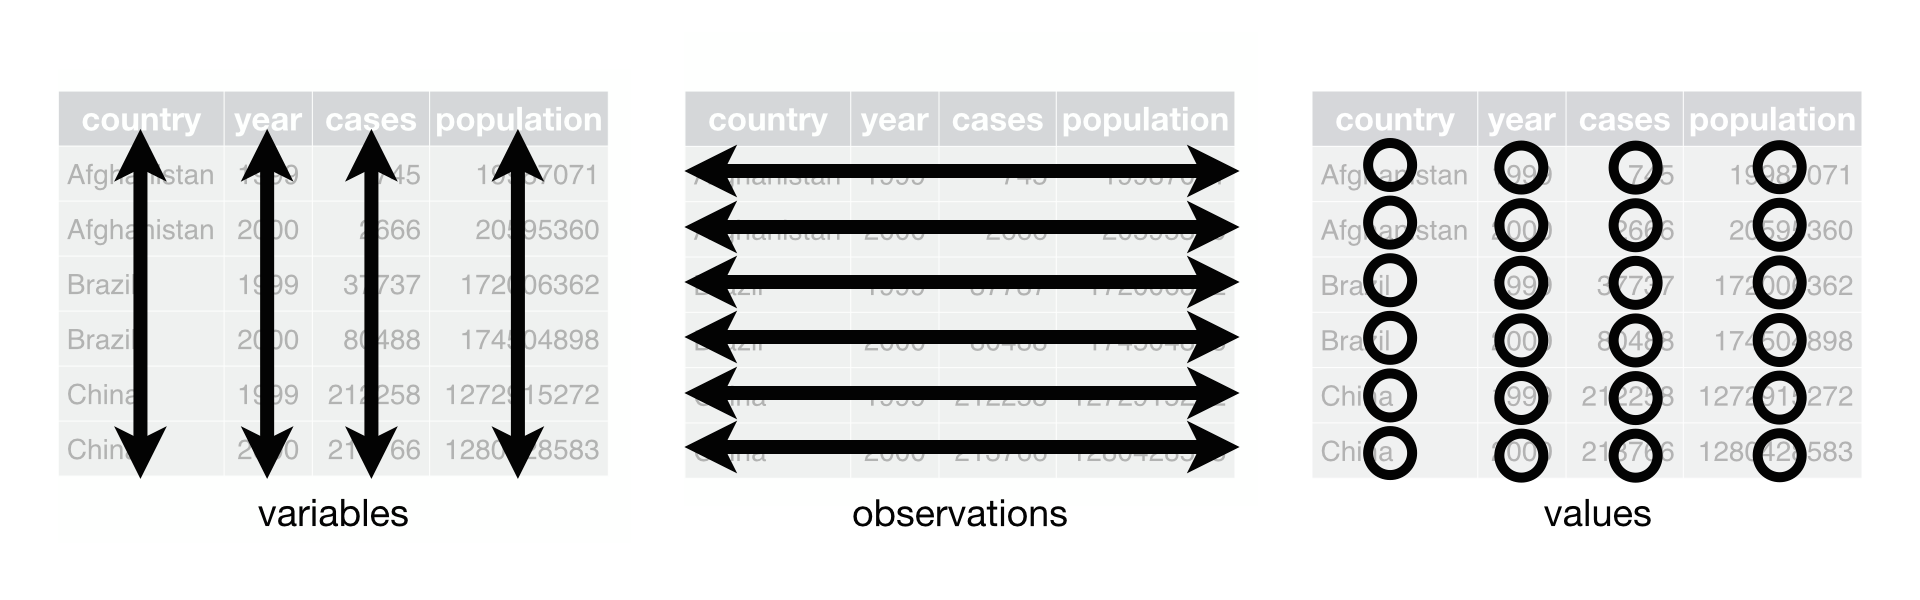
\includegraphics[width=1\textwidth,height=\textheight]{Intro_R_files/mediabag/tidy1.png}

\marginnote{\begin{footnotesize}

Source: R for Data Science. Grolemund and Wickham.

\end{footnotesize}}

\subsection{Pipe operator}\label{pipe-operator}

\begin{itemize}
\item
  One of the key features of tidyverse is the possibility to chain
  functions in an effective way using the pipe operator
  \texttt{\textbar{}\textgreater{}}.
\item
  Pipes pass the results from one function directly into the next
  function connected to each other via a
  \texttt{\textbar{}\textgreater{}}, making the code easy to read and
  write.
\item
  \textbf{The pipe basically means ``and then''.}
\item
  \textbf{Note:} the keyboard shorcut for
  \texttt{\textbar{}\textgreater{}} is \texttt{Ctrl+Shift+M} (Windows \&
  Linux) or \texttt{Cmd+Shift+M} (Mac).
\end{itemize}

\subsection{Pipe operator}\label{pipe-operator-1}

\emph{First, I'll grab the coffee grounds, then I'll fill up the coffee
maker with water, hit the start button, wait for it to brew, and finally
pour myself a cup}

\begin{Shaded}
\begin{Highlighting}[]
\FunctionTok{get}\NormalTok{(}\StringTok{"coffee\_groundS"}\NormalTok{,}\StringTok{"23"}\NormalTok{)  }\SpecialCharTok{|\textgreater{}} 
  \FunctionTok{fill\_up}\NormalTok{(}\StringTok{"coffee\_maker"}\NormalTok{,}\StringTok{"water"}\NormalTok{)   }\SpecialCharTok{|\textgreater{}} 
  \FunctionTok{on}\NormalTok{(start\_button)  }\SpecialCharTok{|\textgreater{}} 
  \FunctionTok{put}\NormalTok{(cup)}
\end{Highlighting}
\end{Shaded}

\subsection{Iris dataset}\label{iris-dataset}

The iris
\href{https://en.wikipedia.org/wiki/Iris_flower_data_set}{flower
dataset} was collected by Edgar Anderson, an American botanist, in the
1920s. This data was used by statistician Ronald Fisher to demonstrate
statistical methods of classification.

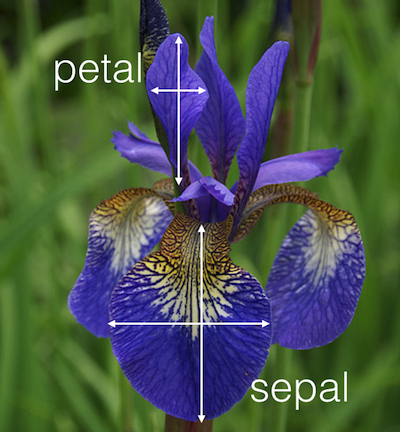
\includegraphics[width=1\textwidth,height=\textheight]{Intro_R_files/mediabag/iris_flower.png}

\subsection{Importing data in R}\label{importing-data-in-r}

R can import data from files in many different formats. For example:

\begin{itemize}
\tightlist
\item
  csv files with the \texttt{readr} package
\item
  excel files with the \texttt{readxl} package
\item
  xlm files with the \texttt{xml2} package
\item
  netcdf files with the \texttt{ncdf4} package
\item
  shapefiles with the \texttt{sf} package
\end{itemize}

\subsection{Formats}\label{formats}

\begin{longtable}[]{@{}lll@{}}
\toprule\noalign{}
Function & Value Separator & Decimal Separator \\
\midrule\noalign{}
\endhead
\bottomrule\noalign{}
\endlastfoot
read\_csv() & , & . \\
read\_csv2() & ; & , \\
read\_tsv() & tab & . \\
read\_delim() & custom character & . \\
read\_table2() & space & . \\
\end{longtable}

\subsection{Reading data}\label{reading-data}

\begin{Shaded}
\begin{Highlighting}[numbers=left,,]
\FunctionTok{library}\NormalTok{(tidyverse)}
\end{Highlighting}
\end{Shaded}

\begin{verbatim}
-- Attaching core tidyverse packages ------------------------ tidyverse 2.0.0 --
v dplyr     1.1.4     v readr     2.1.5
v forcats   1.0.0     v stringr   1.5.1
v ggplot2   3.5.0     v tibble    3.2.1
v lubridate 1.9.3     v tidyr     1.3.1
v purrr     1.0.2     
-- Conflicts ------------------------------------------ tidyverse_conflicts() --
x dplyr::filter() masks stats::filter()
x dplyr::lag()    masks stats::lag()
i Use the conflicted package (<http://conflicted.r-lib.org/>) to force all conflicts to become errors
\end{verbatim}

\begin{Shaded}
\begin{Highlighting}[numbers=left,,]
\NormalTok{iris }\OtherTok{\textless{}{-}} \FunctionTok{read\_csv}\NormalTok{(}\StringTok{"Data/iris.csv"}\NormalTok{)}
\end{Highlighting}
\end{Shaded}

\begin{verbatim}
New names:
Rows: 150 Columns: 6
-- Column specification
-------------------------------------------------------- Delimiter: "," chr
(1): Species dbl (5): ...1, Sepal.Length, Sepal.Width, Petal.Length,
Petal.Width
i Use `spec()` to retrieve the full column specification for this data. i
Specify the column types or set `show_col_types = FALSE` to quiet this message.
* `` -> `...1`
\end{verbatim}

\begin{Shaded}
\begin{Highlighting}[]
\CommentTok{\# R basic function}
\NormalTok{iris }\OtherTok{\textless{}{-}}\FunctionTok{read.csv}\NormalTok{(}\StringTok{"Data/iris.csv"}\NormalTok{)}
\end{Highlighting}
\end{Shaded}

\subsection{Exploring the data}\label{exploring-the-data}

Check that your data was imported without any mistakes

\begin{Shaded}
\begin{Highlighting}[]
\FunctionTok{head}\NormalTok{(iris)    }\CommentTok{\# Displays the first rows of a df}
\end{Highlighting}
\end{Shaded}

\begin{verbatim}
# A tibble: 6 x 6
   ...1 Sepal.Length Sepal.Width Petal.Length Petal.Width Species
  <dbl>        <dbl>       <dbl>        <dbl>       <dbl> <chr>  
1     1          5.1         3.5          1.4         0.2 setosa 
2     2          4.9         3            1.4         0.2 setosa 
3     3          4.7         3.2          1.3         0.2 setosa 
4     4          4.6         3.1          1.5         0.2 setosa 
5     5          5           3.6          1.4         0.2 setosa 
6     6          5.4         3.9          1.7         0.4 setosa 
\end{verbatim}

\begin{Shaded}
\begin{Highlighting}[]
\FunctionTok{tail}\NormalTok{(iris)  }\CommentTok{\# Displays the last rows of a df}
\end{Highlighting}
\end{Shaded}

\begin{verbatim}
# A tibble: 6 x 6
   ...1 Sepal.Length Sepal.Width Petal.Length Petal.Width Species  
  <dbl>        <dbl>       <dbl>        <dbl>       <dbl> <chr>    
1   145          6.7         3.3          5.7         2.5 virginica
2   146          6.7         3            5.2         2.3 virginica
3   147          6.3         2.5          5           1.9 virginica
4   148          6.5         3            5.2         2   virginica
5   149          6.2         3.4          5.4         2.3 virginica
6   150          5.9         3            5.1         1.8 virginica
\end{verbatim}

\subsection{Exploring the data}\label{exploring-the-data-1}

\begin{Shaded}
\begin{Highlighting}[]
\FunctionTok{glimpse}\NormalTok{(iris) }\CommentTok{\# Tells you variables types }
\end{Highlighting}
\end{Shaded}

\begin{verbatim}
Rows: 150
Columns: 6
$ ...1         <dbl> 1, 2, 3, 4, 5, 6, 7, 8, 9, 10, 11, 12, 13, 14, 15, 16, 17~
$ Sepal.Length <dbl> 5.1, 4.9, 4.7, 4.6, 5.0, 5.4, 4.6, 5.0, 4.4, 4.9, 5.4, 4.~
$ Sepal.Width  <dbl> 3.5, 3.0, 3.2, 3.1, 3.6, 3.9, 3.4, 3.4, 2.9, 3.1, 3.7, 3.~
$ Petal.Length <dbl> 1.4, 1.4, 1.3, 1.5, 1.4, 1.7, 1.4, 1.5, 1.4, 1.5, 1.5, 1.~
$ Petal.Width  <dbl> 0.2, 0.2, 0.2, 0.2, 0.2, 0.4, 0.3, 0.2, 0.2, 0.1, 0.2, 0.~
$ Species      <chr> "setosa", "setosa", "setosa", "setosa", "setosa", "setosa~
\end{verbatim}

\begin{Shaded}
\begin{Highlighting}[]
\FunctionTok{summary}\NormalTok{(iris) }\CommentTok{\# Gives you a summary of the data}
\end{Highlighting}
\end{Shaded}

\begin{verbatim}
      ...1         Sepal.Length    Sepal.Width     Petal.Length  
 Min.   :  1.00   Min.   :4.300   Min.   :2.000   Min.   :1.000  
 1st Qu.: 38.25   1st Qu.:5.100   1st Qu.:2.800   1st Qu.:1.600  
 Median : 75.50   Median :5.800   Median :3.000   Median :4.350  
 Mean   : 75.50   Mean   :5.843   Mean   :3.057   Mean   :3.758  
 3rd Qu.:112.75   3rd Qu.:6.400   3rd Qu.:3.300   3rd Qu.:5.100  
 Max.   :150.00   Max.   :7.900   Max.   :4.400   Max.   :6.900  
  Petal.Width      Species         
 Min.   :0.100   Length:150        
 1st Qu.:0.300   Class :character  
 Median :1.300   Mode  :character  
 Mean   :1.199                     
 3rd Qu.:1.800                     
 Max.   :2.500                     
\end{verbatim}

\subsection{Manipulating data}\label{manipulating-data}

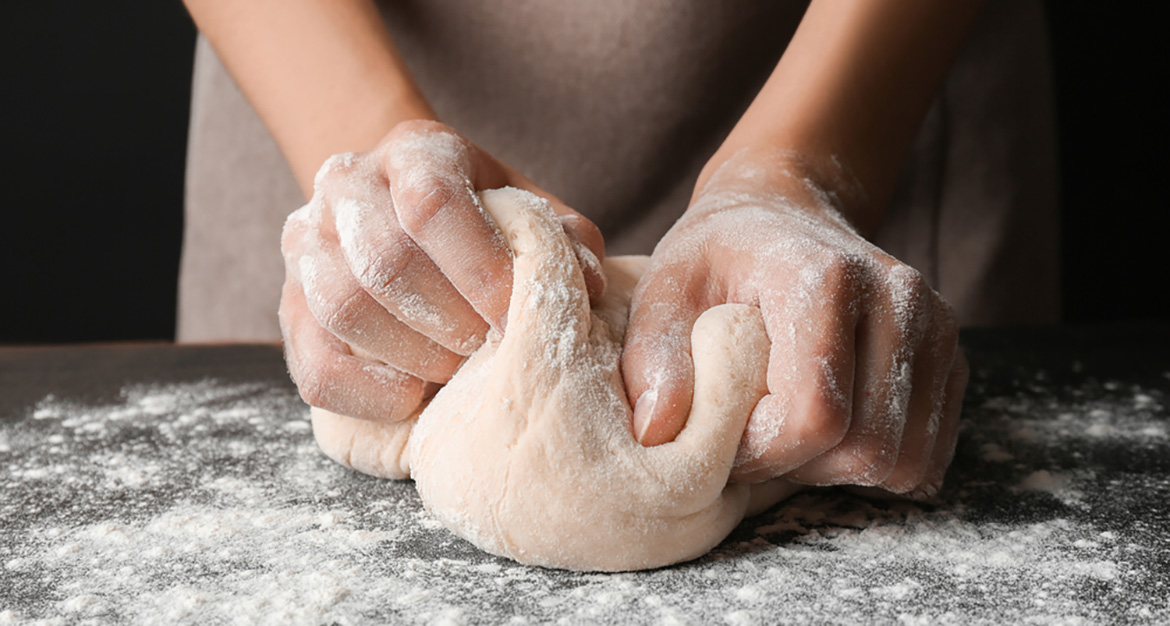
\includegraphics[width=0.8\textwidth,height=\textheight]{Intro_R_files/mediabag/person-making-fresh-.jpg}

\subsection{From wide to long}\label{from-wide-to-long}

The iris data are organized is ``wide'' format. Let's transform in
``long'' format

\begin{Shaded}
\begin{Highlighting}[]
\NormalTok{iris\_long }\OtherTok{\textless{}{-}}\NormalTok{ iris }\SpecialCharTok{|\textgreater{}} \FunctionTok{pivot\_longer}\NormalTok{( }
                    \AttributeTok{cols =} \SpecialCharTok{{-}}\NormalTok{Species,}
                    \AttributeTok{names\_to =} \StringTok{"trait"}\NormalTok{,}
                    \AttributeTok{values\_to =} \StringTok{"measurement"}\NormalTok{)}
\FunctionTok{head}\NormalTok{(iris\_long)}
\end{Highlighting}
\end{Shaded}

\begin{verbatim}
# A tibble: 6 x 3
  Species trait        measurement
  <chr>   <chr>              <dbl>
1 setosa  ...1                 1  
2 setosa  Sepal.Length         5.1
3 setosa  Sepal.Width          3.5
4 setosa  Petal.Length         1.4
5 setosa  Petal.Width          0.2
6 setosa  ...1                 2  
\end{verbatim}

\subsection{Group\_by and summarize}\label{group_by-and-summarize}

\begin{Shaded}
\begin{Highlighting}[]
\NormalTok{iris\_means }\OtherTok{\textless{}{-}}\NormalTok{ iris }\SpecialCharTok{|\textgreater{}} 
  \FunctionTok{group\_by}\NormalTok{(Species) }\SpecialCharTok{|\textgreater{}} 
  \FunctionTok{summarize}\NormalTok{(}\AttributeTok{SL\_mean =} \FunctionTok{mean}\NormalTok{(Sepal.Length),}
            \AttributeTok{SL\_se =} \FunctionTok{sd}\NormalTok{(Sepal.Length)}\SpecialCharTok{/}\FunctionTok{sqrt}\NormalTok{(}\FunctionTok{n}\NormalTok{()))}

\FunctionTok{head}\NormalTok{(iris\_means)}
\end{Highlighting}
\end{Shaded}

\begin{verbatim}
# A tibble: 3 x 3
  Species    SL_mean  SL_se
  <chr>        <dbl>  <dbl>
1 setosa        5.01 0.0498
2 versicolor    5.94 0.0730
3 virginica     6.59 0.0899
\end{verbatim}

\subsection{Filter - subset rows}\label{filter---subset-rows}

\begin{Shaded}
\begin{Highlighting}[]
\NormalTok{iris\_versicolor }\OtherTok{\textless{}{-}}\NormalTok{ iris }\SpecialCharTok{|\textgreater{}}  \FunctionTok{filter}\NormalTok{( Species }\SpecialCharTok{==} \StringTok{"versicolor"}\NormalTok{)}

\NormalTok{iris\_no\_versicolor }\OtherTok{\textless{}{-}}\NormalTok{ iris }\SpecialCharTok{|\textgreater{}}  \FunctionTok{filter}\NormalTok{( Species }\SpecialCharTok{!=} \StringTok{"versicolor"}\NormalTok{)}

\NormalTok{iris\_pl}\OtherTok{\textless{}{-}}\NormalTok{iris }\SpecialCharTok{|\textgreater{}}  \FunctionTok{filter}\NormalTok{(Petal.Length }\SpecialCharTok{\textgreater{}} \DecValTok{2}\NormalTok{)}
\end{Highlighting}
\end{Shaded}

\subsection{Select - subset columns}\label{select---subset-columns}

\begin{Shaded}
\begin{Highlighting}[]
\NormalTok{iris\_subset}\OtherTok{\textless{}{-}}\NormalTok{iris }\SpecialCharTok{|\textgreater{}} \FunctionTok{select}\NormalTok{(Species, Petal.Width, Petal.Length)}
\end{Highlighting}
\end{Shaded}

\subsection{Mutate}\label{mutate}

\begin{Shaded}
\begin{Highlighting}[]
\NormalTok{iris\_log }\OtherTok{\textless{}{-}}\NormalTok{iris }\SpecialCharTok{|\textgreater{}} \FunctionTok{mutate}\NormalTok{(}\AttributeTok{log.Sepal.length =} \FunctionTok{log}\NormalTok{(Sepal.Length))}

\FunctionTok{head}\NormalTok{(iris\_log)}
\end{Highlighting}
\end{Shaded}

\begin{verbatim}
# A tibble: 6 x 7
   ...1 Sepal.Length Sepal.Width Petal.Length Petal.Width Species
  <dbl>        <dbl>       <dbl>        <dbl>       <dbl> <chr>  
1     1          5.1         3.5          1.4         0.2 setosa 
2     2          4.9         3            1.4         0.2 setosa 
3     3          4.7         3.2          1.3         0.2 setosa 
4     4          4.6         3.1          1.5         0.2 setosa 
5     5          5           3.6          1.4         0.2 setosa 
6     6          5.4         3.9          1.7         0.4 setosa 
# i 1 more variable: log.Sepal.length <dbl>
\end{verbatim}

\subsection{Plotting data}\label{plotting-data}

You can plot graphs using the ggplot2 package (part of the tidyverse).

\textbf{Note:} \texttt{ggplot} functions are chained using a \texttt{+}
sign. This is because \texttt{ggplot} does not pass an object to a
function but add different layers on top of each other.

\subsection{ggplot layers}\label{ggplot-layers}

\begin{figure}[H]

{\centering 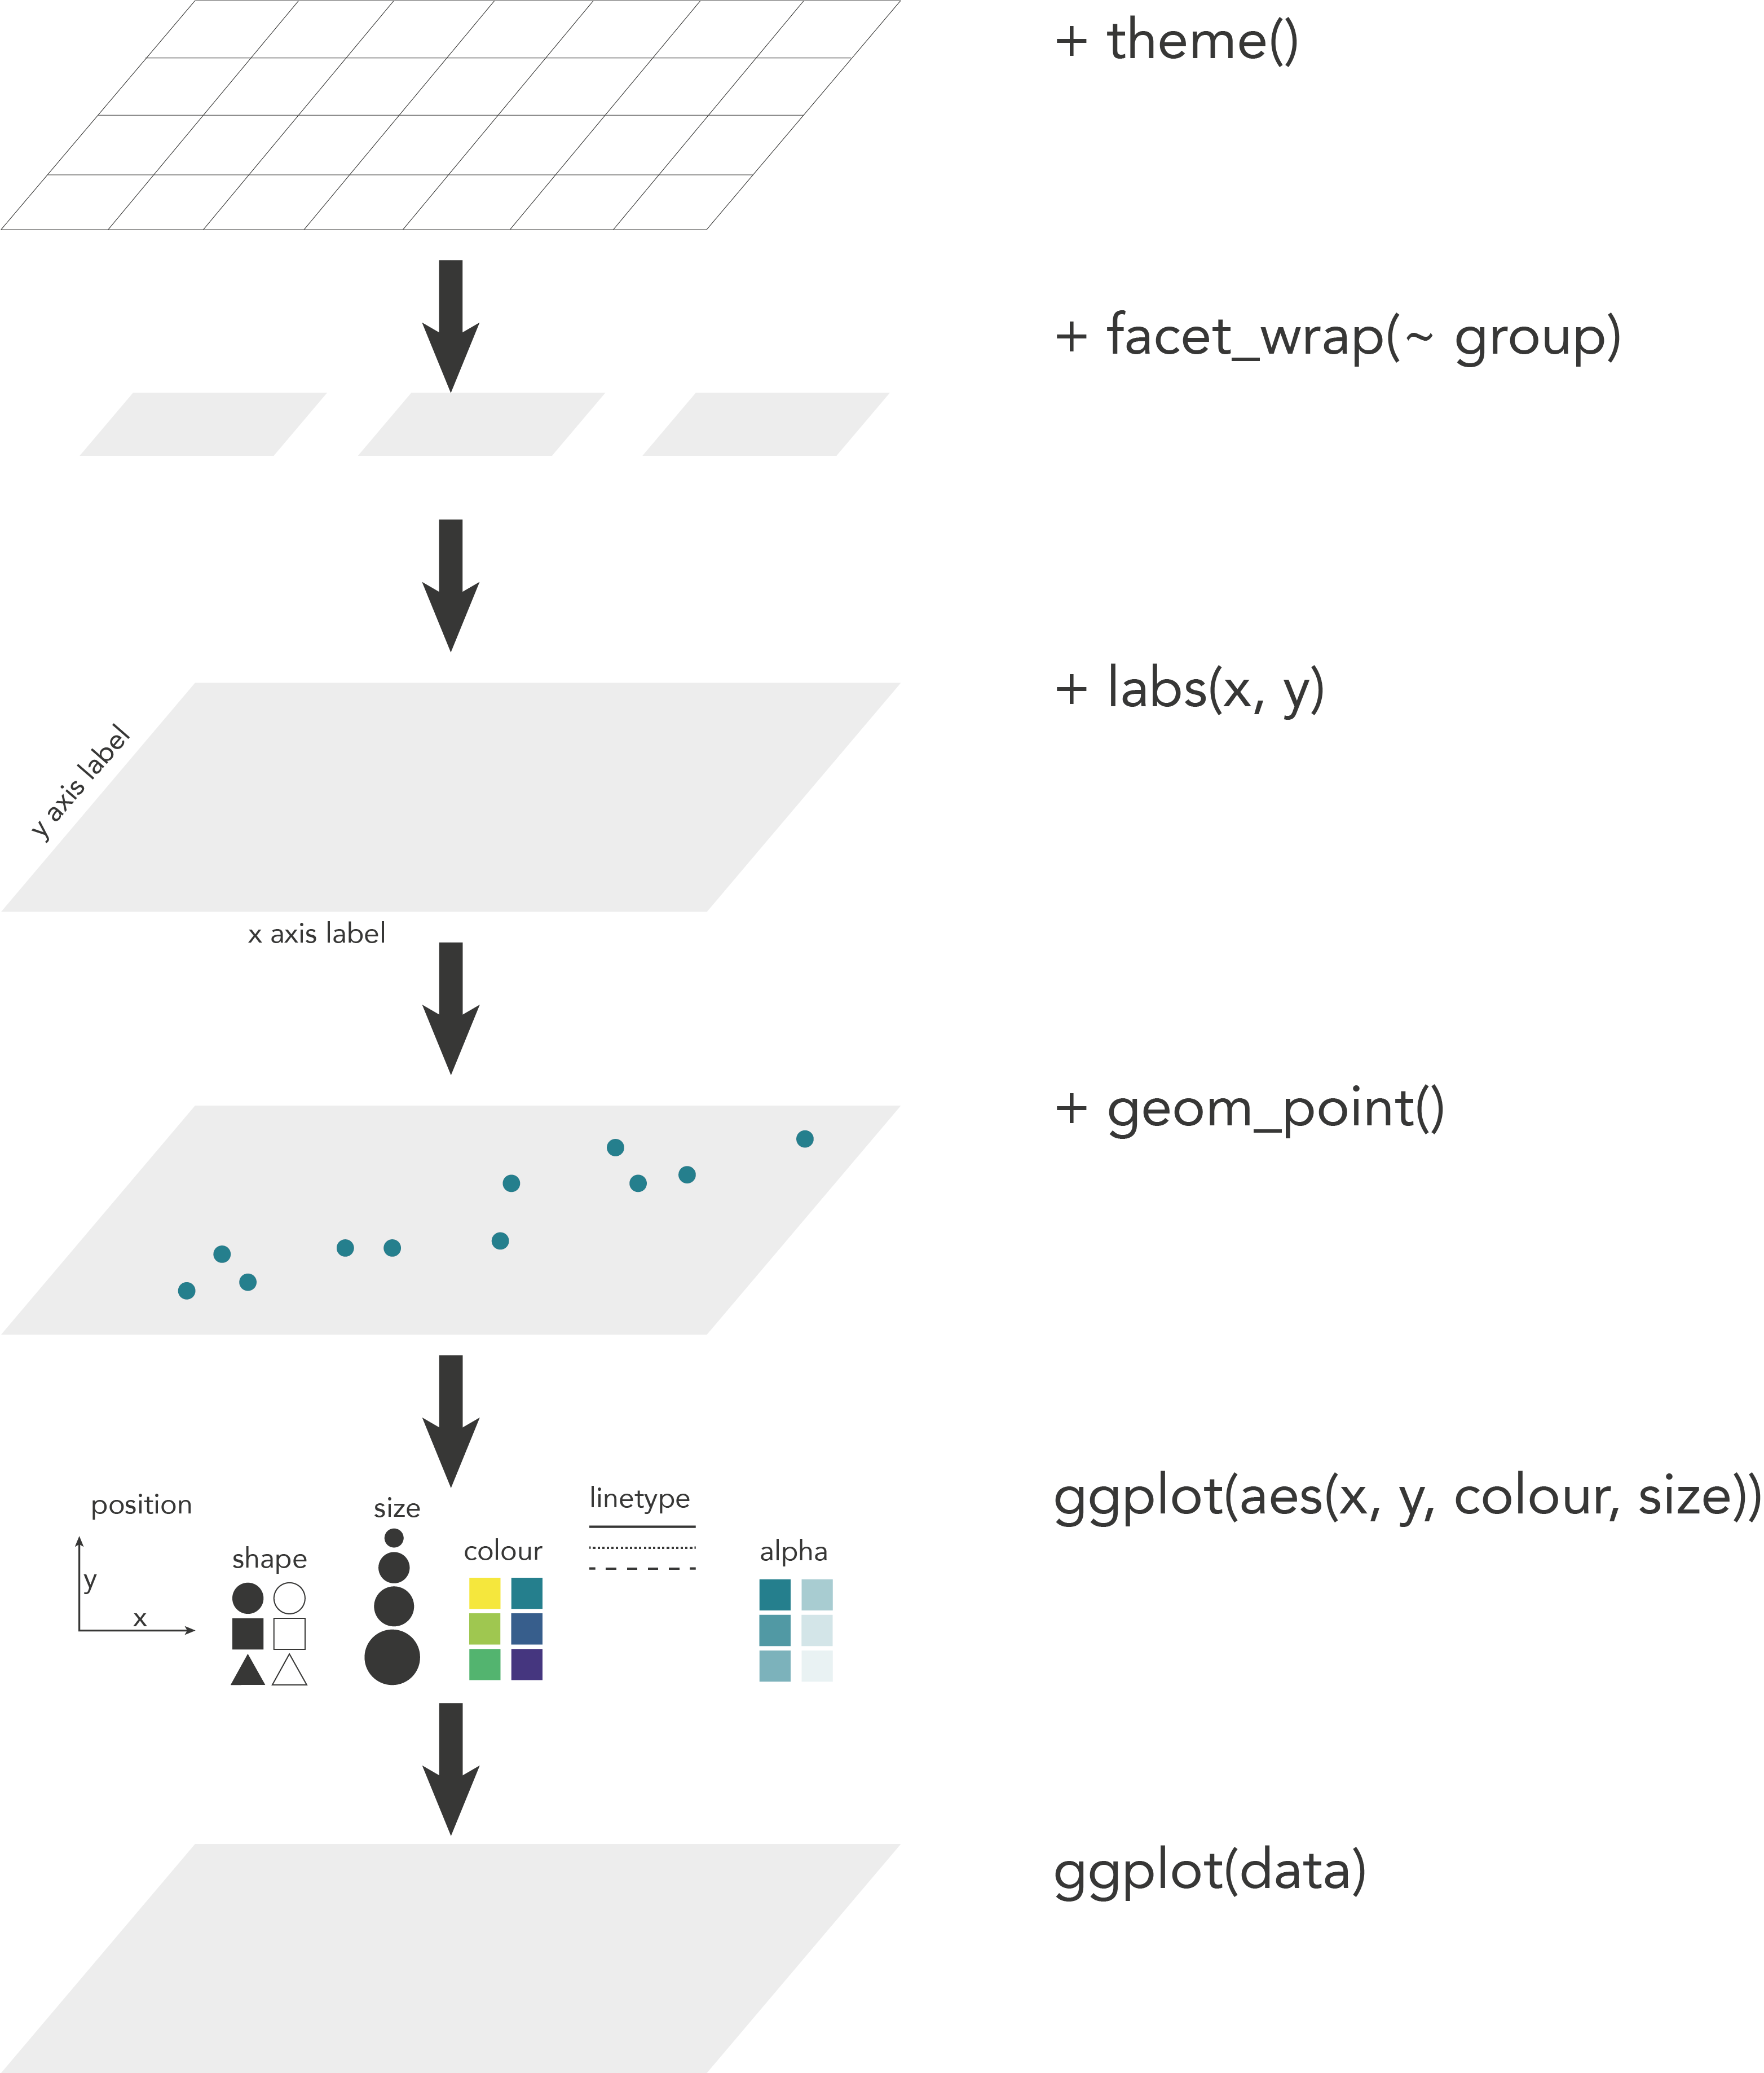
\includegraphics[width=0.6\textwidth,height=\textheight]{Intro_R_files/mediabag/ggplot_setup.png}

}

\caption{Source: https://biostats-r.github.io/}

\end{figure}%

\subsection{Plotting Iris}\label{plotting-iris}

Lets say we want to plot the relationship between petal length and petal
width for each species.

You can visualize such relationship by plotting petal length against
petal width in a scatter plot:

\begin{Shaded}
\begin{Highlighting}[]
\NormalTok{iris }\SpecialCharTok{\%\textgreater{}\%} 
  \FunctionTok{ggplot}\NormalTok{(}\FunctionTok{aes}\NormalTok{(}
    \AttributeTok{x =}\NormalTok{ Petal.Length,}
    \AttributeTok{y =}\NormalTok{ Petal.Width,}
    \AttributeTok{color =}\NormalTok{ Species }\CommentTok{\# to assign a color to each group}
\NormalTok{  )) }\SpecialCharTok{+}
  \FunctionTok{geom\_point}\NormalTok{() }\SpecialCharTok{+} \CommentTok{\# to plot a scatter plot}
  \FunctionTok{labs}\NormalTok{(}
    \AttributeTok{x =} \StringTok{"Petal length (cm)"}\NormalTok{,}
    \AttributeTok{y =} \StringTok{"Petal width (cm)"}
\NormalTok{  )}
\end{Highlighting}
\end{Shaded}

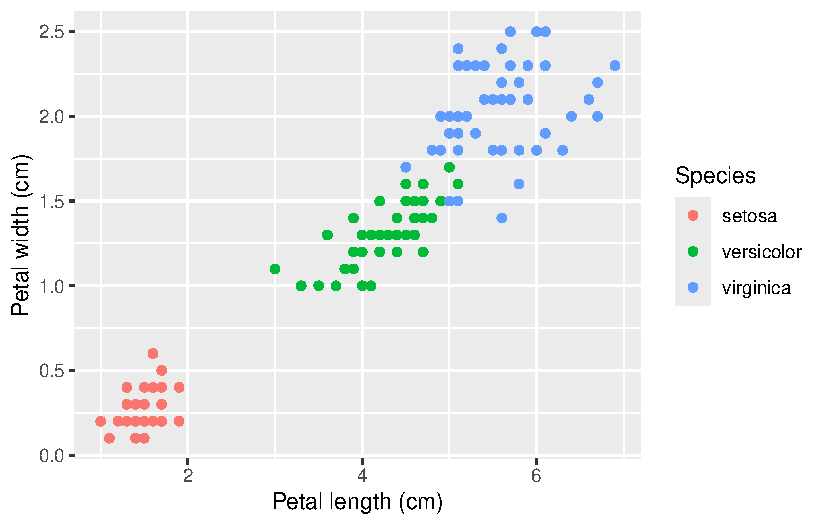
\includegraphics{Intro_R_files/figure-pdf/unnamed-chunk-22-1.pdf}

\subsection{Plotting Iris}\label{plotting-iris-1}

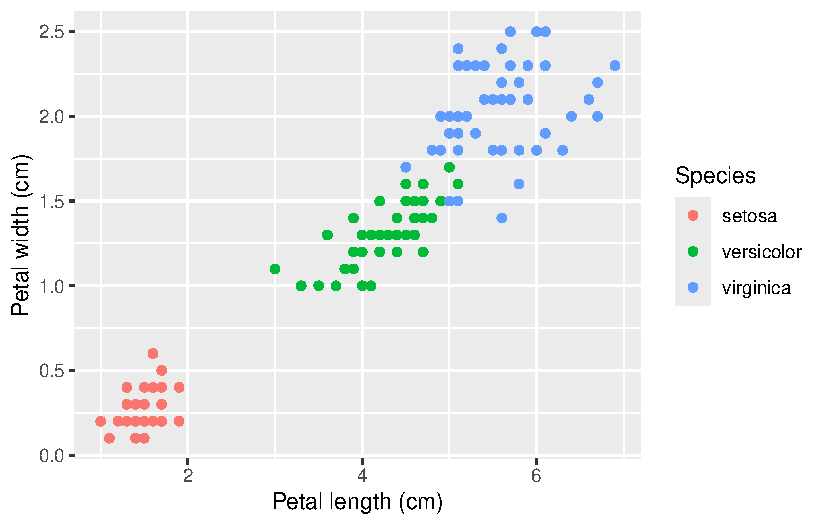
\includegraphics{Intro_R_files/figure-pdf/unnamed-chunk-23-1.pdf}

\subsection{Modelling}\label{modelling}

\subsection{Saving plots}\label{saving-plots}

You can save a plot by clicking on the \texttt{Export} button in the
\texttt{Plots} window (bottom right window by default).

Save your plots as \texttt{.svg} if your text editor supports it and if
you are not limited by file sizes. Otherwise, save your plots as
\texttt{.png}.

\begin{Shaded}
\begin{Highlighting}[]
\NormalTok{plot }\SpecialCharTok{|\textgreater{}} \FunctionTok{ggsave}\NormalTok{(}\StringTok{"plot.png"}\NormalTok{)}
\end{Highlighting}
\end{Shaded}

\subsection{To go further}\label{to-go-further}

Visit: \href{https://ourcodingclub.github.io/}{Coding Club}



\end{document}
